% This is samplepaper.tex, a sample chapter demonstrating the
% LLNCS macro package for Springer Computer Science proceedings;
% Version 2.20 of 2017/10/04
%
\documentclass[runningheads]{llncs}
%
\usepackage{graphicx}
% Used for displaying a sample figure. If possible, figure files should
% be included in EPS format.
%
% If you use the hyperref package, please uncomment the following line
% to display URLs in blue roman font according to Springer's eBook style:
% \renewcommand\UrlFont{\color{blue}\rmfamily}
\graphicspath{ {images/} }

\begin{document}
%
\title{\textbf{Java Path Finder}
}
%
%\titlerunning{Abbreviated paper title}
% If the paper title is too long for the running head, you can set
% an abbreviated paper title here
%
\author{Farias Juan Ignacio\and
Kokic Emiliano\and
Moresi Marco}
%
\authorrunning{Farias Juan - Kokic Emiliano - Moresi Marco}
% First names are abbreviated in the running head.
% If there are more than two authors, 'et al.' is used.
%
\institute{Facultad de Matem\'atica, Astronom\'ia, F\'isica y Computaci\'on, C\'ordoba, Argentina}
%
\maketitle              % typeset the header of the contribution
%
\begin{abstract}
Esta investigación fue centrada en el funcionamiento de la herramienta Java Path Finder, la cual permite verificar programas escritos en Java. Se investigó sobre distintos aspectos técnicos de la misma como así también aspectos de usabilidad e interacción con el usuario.
Dado lo versátil de la herramienta, decidimos acotar la investigación sólo al uso de JPF como model checker de programas concurrentes. Esta investigación aporta un análisis para aquellos nuevos usuarios de esta herramienta desarrollada por la NASA y hoy de código abierto.


\keywords{JPF \and Model Checker \and Java.}
\end{abstract}
%
%
%
\section{Contexto de creación de la herramienta}

Java Path Finder, también como conocido como JPF,  se comenzó a desarrollar en el año  1999 como un traductor de Java a Promela (usando Spin como model checker). Para el año 2000, se convirtió en una herramienta de model checker por si sola, dejando de lado la utilización de Spin. Las primeras etapas fueron desarrolladas por el grupo Robust Software Engineering en la NASA Ames Research Center, junto con el apoyo de organizaciones tales como RIACS (The Research Institute for Advanced Computer Science).
En el año 2005 se convirtió en una herramienta de código abierto. Actualmente, se encuentra disponible de manera gratuita y en desarrollo continuo gracias al apoyo de más de 20 universidades de todo el mundo.

\begin{figure}
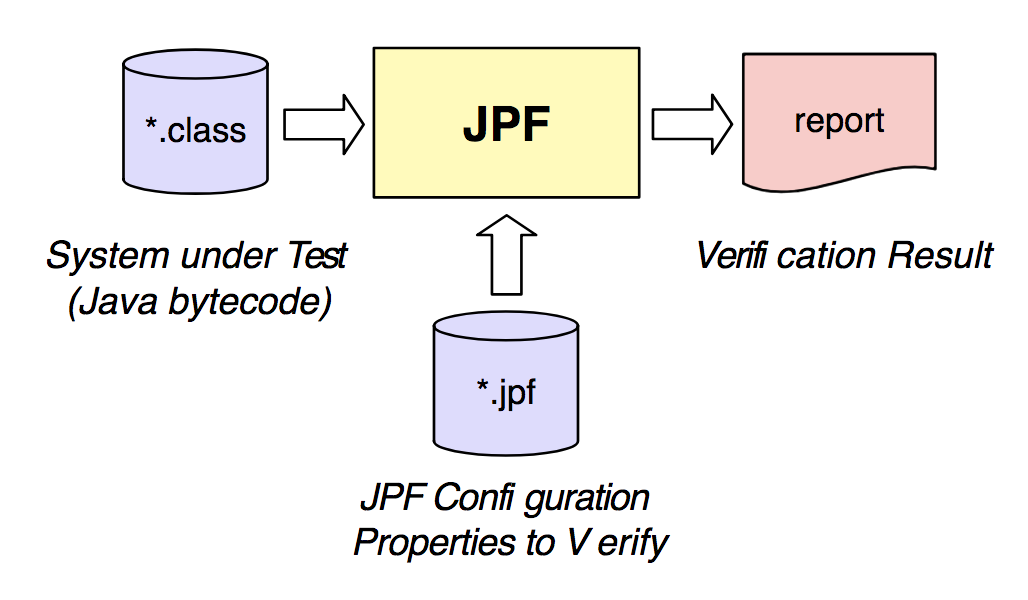
\includegraphics[width=\textwidth]{fig1.png}
\caption{The Core : a VM that supports Model Checking} \label{fig1}
\end{figure}

\section{Objetivo de la herramienta}



El objetivo de JPF depende como se configure la herramienta, el núcleo principal de JPF es una Java Virtual Machine que ejecuta código compilado de Java (Java Bytecode). Es utilizado para detectar defectos, para lo cual, JPF toma como entrada el programa a verificar y la configuración que se desea verificar (archivo .jpf). JPF devolverá un reporte describiendo si las propiedades de la configuración se mantienen y/o que artefactos de verificación han sido creados por JPF para su posterior análisis. 
Un conjunto de instrucciones por defecto hace uso de una caracteristica importante de JPF: execution choices. JPF puede identificar puntos en el programa donde la ejecuci\'on puede proceder de diferentes maneras, luego explora sistematicamente cada uno de estos puntos, es decir, JPF ejecuta todos los paths. En cuanto al numero de paths, puede crecer exponencialmente (esto es llamado como state explosion problem). Para lidiar con esto, JPF emplea una linea de defensa llamada state matching: cada vez que JPF alcanza un choice point, checkea si ya ha visto un estado similar en el programa y en tal caso, abandona ese path, realiza un backtrack a un choice point previo que tenga choices no exploradas y procede desde alli. 
En caso de ejecutar sin una configuración propia, por defecto JPF verificará el programa en búsqueda de deadlocks y excepciones no controladas (unhandled exceptions). Estas son llamadas propiedades non-funcional. Pero como se menciono previamente, el usuario puede definir propiedades espec\'ificas, que en su mayoria, se realizan con los llamados listeners (pequeños ‘plugins’ que permiten monitorear con mas detalle todas las acciones que va tomando JPF). Todo explica porque JPF es llamado "a debugger toolbox on steroids", primero automáticamente ejecuta el programa de entrada en todas sus formas posibles para detectar defectos y cuando los encuentra muestra una explicación de que lo causó.


\section{Descripción de la herramienta del lado del usuario}

JPF no presenta interfaz gráfica propia, pero permite ser ejecutado de diversas maneras. Se puede utilizar desde la linea de comandos, como asi tambi\'en desde los diversos IDE de desarrollo para Java como NetBeans o Eclipse donde es necesario instalar los plugins correspondientes. Como si esto fuera poco se puede integrar JPF al programa de Java como una clase embebida.
Además se puede ejecutar desde JUnit el framework de java para escribir Unit Test.


\section{Aspectos técnicos de la herramienta}

JPF fue diseñanda en base a dos abstracciones, la VM (máquina virtual), y Search Component.
La encargada de generar los estados es la VM, mediante la ejecución de instrucciones en Java Byte Code, la VM  genera la representación de los estados, los cuales pueden ser:

\begin{itemize}
\item Verificados por igualdad (es decir, si el estado ha sido visitado antes).
\item Analizados (ver los valores que contiene).
\item Almacenados.
\item Restaurados.
\end{itemize}

Search Component es el responsable de elegir el siguiente estado que se ejecutará, la ejecuci\'on puede ser parametrizada: $forward$, genera el siguiente estado y reporta si el mismo tiene sucesor (en caso de tener sucesor, guardará el estado en una pila backtrack), $backtrack$, restaura el último estado en la pila backtrack, $restoreState$ restaura un estado arbitrario (no necesariamente de la pila backtrack).

Más aún puede ser configurado para usar diferentes estrategias de búsqueda tales como DFS, cola de prioridades, entre otros.
El número de las diferentes combinaciones de scheduling crece exponencialmente a medida que crecen los programas. Para atacar esta dificultad JPF implementa $Partial Order Reduction (POR)$, esta técnica consta de agrupar todas las instrucciones en un thread que no tienen efecto en otros threads, de modo que sea una sola transición en el sistema de estados. Esta técnica suele reducir el espacio de estados en un 70\%.
Si $POR$ está habilitado, la máquina virtual ejecutará todo el thread en caso de recibir un request forward hasta que ocurra alguna de las siguientes posibilidades: la siguiente instrucción es relevante para el scheduling o bien la siguiente instrucción contiene un resultado no determinístico.

JPF tiene manejo explícito de estados, lo realiza creando instancias de la clase SystemState para encapsular información relevante para la ejecución: tales como estado del thread, pila, cola, valores de las variables locales, entre otra información.


\section{Casos de estudio (exitosos o no) de la herramienta}

Los primeros usos que se le dio a esta herramienta fueron para proyectos de la NASA, dado que era privativo el software, entre ellos se destacan proyectos como la verificación del software del NASA Ames K9 Rover [3] que es una plataforma para vehículos autónomos para reconocimiento de suelo de planetas tales como Marte.
Otro uso significativo, por parte de la NASA, fue usarlo para traducir gráficos de estados UML, permitiendo así una relación uno a uno con el modelo en UML y código escrito en Java, que es más fácil de leer [4].\\
A su vez, fue utilizado en un sistema para aviones comerciales (The DEOS Avionics Operating System), implementado en C++. Este sistema fue llevado a la NASA para su verificación, siendo necesarias, además de la traducción a Java, t\'ecnicas de reducci\'on de estados como $POR$, ya que de otra manera el error no era encontrado.\\
También se puede mencionar, el uso de esta herramienta por la empresa japonesa Fujitsu (3ra en ranking de empresas de IT), la cual uso JPF, en modo simbólico (SPF), para analizar una cantidad de datos masiva.
Por último, podemos mencionar la existencia de muchos casos de estudios realizados en Google Summer of Code, donde un estudiante realiza un proyecto con la ayuda de su mentor, utilizando JPF. Algunos de los proyectos que podemos mencionar son: 
JPF for android Devices es un proyecto de Google Summer of Code 2016 que pretende incorporar JPF en android, brindando tecnicas de verificacion para encontrar bugs en aplicaciones android.
Extending SPF es una herramienta de ejecucion simbolica basada en JPF. Ejecuta el JavaBytecode usando un JVM personalizada para realizar su analisis.


\section{Comparación con otras herramientas}

JPF al trabajar con Java Bytecode, no requiere traducir ni armar otros modelos, algo que si se debe hacer en LTSA por ejemplo. En otras herramientas, es comun seleccionar propiedades (ya implementadas) que se quieran analizar, cosa que en JPF no sucede ya que se deben implementar (a no ser que se seleccione alguna que viene por defecto).

Otra diferencia a destacar, es que en LTSA se debe definir el algebra FSP de lo que se quiere modelar, mientras que JPF crea el modelo directamente a partir del codigo Java.

\section{Caso de estudio elegido}

A continuacion explicaremos el caso de estudio elegido, donde el objetivo del mismo fue comparar 3 tecnicas diferentes (Model Checking(MC), Runtime Analysis(RA) y Testing(TT)), para detectar bugs como Deadlocks, Data Race y Plan Semantics sobre 3 versiones del codigo del NASA Ames K9 Rover,el cual es una plataforma para vehículos autónomos para reconocimiento de suelo de planetas tales como Marte.
Dada la complejidad de crear un experimento como este, resulta imposible reportar conclusiones validas de manera estatica, por eso solo se concentraron en los resultados de MC, RA y TT. Cabe destacar que la herramienta utilizada para realizar MC fue JPF, y que es esta sobre la cual mas queremos centrarnos, aunque el analisis que se realiza en este caso de estudio surge de la comparacion con las otras tecnicas mencionadas.
La figura(SACAR IMAGEN DEL PAPER  Figura 3) muestra como se desempeñaron las diferentes tecnicas en la busqueda de errores. Las tecnicas mas avanzadas como MC y RA resultaron ser mas eficientes en los errores relacionados a la concurrencia. El hecho de que TT haya sido peor que MC en todas las categorias fue un detalle un tanto inesperado.
En la figura(SACAR IMAGEN DEL PAPER  Figura 4) se puede observar el detalle por dia de los bugs encontrados en una linea de tiempo de 48 horas (3 sesiones de 2 dias, cada dia consistiendo de 8 horas). Una primera observacion sobre MC, es que los Spurious Errors, decrementan a lo largo de las tres versiones. Esto se debe a que los participantes se familiarizan con el codigo y desarrollan mejores abstracciones. Deadlock 3 es simple y fue encontrado rapidamente por los tres metodos. Deadlock 1 es un poco mas complejo pero fue encontrado por MC y RA, aunque TT nunca lo encontró. Deadlock 2 fue el mas complejo y fue encontrado en la ultima version solo por MC. Respecto a los errores de Data Race, el equipo de MC solo intentó encontrar este tipo de errores al final del experimento, por eso solo lo detectó en la ultima version. Un deadlock restante que ningun equipo encontró, era extremadamente sutil y venia luego de un Data Race. A pesar de esto, se contaba con el error debido a que habia sido encontrado por JPF antes de comenzar el experimento.
En las figuras (SACAR FIGURAS 5-7), se puede observar como los participantes del experimento, dedicaron su tiempo en el analisis de las tres versiones diferentes del codigo. Las tres categorias fueron definidas rigurosamente de la siguiente manera:
Delays: incluye espera de hardware y tiempo en solucionar fallas en la tool, como tambien tiempo esperando un feedback.
Setup/Preparation: para el caso de MC incluyó el tiempo en crear las abstracciones, escribir las propiedades y test-cases.
Running the Rover: no fue muy relevante para MC pero si lo fue para RA y TT.
Running the tool: TT no utilizó ninguna tool, pero MC y RA estuvieron basadas en tools.
Result Analysis: este es el tiempo destinado a determinar la causa del error. Para el caso de MC, esto significa determinar si el error es Spurious o no.
La observacion mas notable, es que el equipo de MC utilizo la tool todo el tiempo mientras realizaban otras actividades. Hay menos tiempo dedicado corriendo el Model Checker en la primer version, debido a que todavia no se llega a conocer el problema por completo, pero si es notable el uso del 100% del mismo en la ultima version ya que el problema se hace mucho mas grande. Otra observacion para el equipo de MC, es que dedicaron mucho mas tiempo en Setup en la primer version que en las dos siguientes. Esto da la pauta de que utilizar un Model Checker tal como lo es JPF requiere mas tiempo en crear un entorno ideal.


\section{Conclusiones particulares}

JPF fue desarrollada con el objetivo de que sea una herramienta dinamica y con la posibilidad de extenderla y/o adecuarla segun el analisis o estudio que se quiera realizar. La gran desventaja que tiene es que requiere grandes esfuerzos de configuracion, ya que se se deben setear propiedades, las cuales en muchos casos son dificiles de entender e implementar y al momento de especificar software critico lo es mas aun, aunque en este caso, JPF es la solucion ideal (No es casualidad que sea utilizado por la NASA). Pero todo esto genera que muchos usuarios no lo vean factible al uso de JPF.
No trabaja independientemente, ya que necesita de una terminal o IDEs, configuraciones y modulos especificos para poder ejecutarlo y reportar resultados. Su instalacion no es muy complicada, pero si puede serlo si no se cuenta de antemano con las herramientas que necesita JPF para poder ejecutarse. Al no contar con interfaz grafica propia, se torna mas dificil su uso, aunque lo positivo es que existen plugins que lo hacen menos tedioso.
Como conclusion, mas alla de la complejidad de JPF en su todo, es una herramienta muy completa, que puede solucionar problemas sobre diversos campos de ejecucion, de manera efectiva, segun sus configuraciones y optimizaciones. Ademas, al ser una herramienta que trabaja puramente con java, lo hace mas util y popular aun.


%
% ---- Bibliography ----
%
% BibTeX users should specify bibliography style 'splncs04'.
% References will then be sorted and formatted in the correct style.
%
% \bibliographystyle{splncs04}
% \bibliography{mybibliography}
%
\begin{thebibliography}{8}
\bibitem{ref_url1}
Documentacion anterior\url{https://babelfish.arc.nasa.gov/}.

\bibitem{ref_url1}
Documentacion vigente\url{https://github.com/javapathfinder/jpf-core/wiki}.

\bibitem{ref_url1}
Experimental Evaluation of Verification and Validation Tools on Martian Rover Software.\url{http://sci-hub.tw/10.1023/b:form.0000040027.28662.a4}.

\bibitem{ref_url1}
Trust Your Model - Verifying Aerospace System Models with Java™ Pathfinder.\url{https://ti.arc.nasa.gov/m/pub-archive/1402/1402\%20(Mehlitz).pdf}.

\bibitem{ref_book1}
Willem Visser, Guillaume Brat, Klaus Havelund, SeungJoon Park. Model Checking
Programs. 3–12. 2000

\end{thebibliography}
\end{document}
